% flatex input: [gnd_dn_lambda.tex]

\begin{figure}[h]
\centering
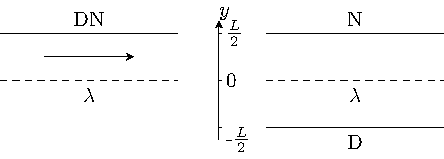
\includegraphics{fig_gnd_dn_lambda.pdf}
\caption{Partition function of Hamiltonian with DN and $\lambda$ boundary conditions. The width of the strip is $\pi$ due to folding. We unfold the cylinder and the new stripe have $N$ and $D$ boundary conditions on the left and right plus a $\lambda$ junction in the middle. }
\end{figure}

{\bf Eigenfunction}: 

The unfolded configuration has D/N boundary conditions at $x = \pm \frac{L}{2}$ and linking boundary condition at $x = 0$. The general solutions can be written as
\begin{equation}
f(k, x) = 
\left\lbrace
\begin{aligned}
  A_1 e^{i kt} \cos(kx +\frac{1}{2}kL ) &  \quad x < 0  \\
  A_2 e^{ikt}  \sin(kx - \frac{1}{2}kL ) & \quad x > 0   \\
\end{aligned} \right. 
\end{equation}
At the junction we have $\frac{\partial_x \phi_1}{ \partial_t \phi_1} = \lambda^2 \frac{\partial_x \phi_2}{ \partial_t \phi_2}$, which cancels the $A$s and gives
\begin{equation}
\tan ^2 (\frac{1}{2} kL ) = \lambda^2 
\end{equation}
Hence
\begin{equation}
 \frac{kL}{2} = \pm \theta + n \pi \implies  k = \frac{2\pi}{L}( n \pm \frac{\theta}{\pi} )  \quad \theta \in [0,\frac{\pi}{2} ]  
\end{equation}
The normalized eigenfunctions are
\begin{equation}
f_n(x) = \sqrt{\frac{2}{L}}
\left\lbrace
\begin{aligned}
  \cos(kx +\frac{1}{2}kL ) &  \quad x < 0  \\
  \pm \sin(kx - \frac{1}{2}kL ) & \quad x > 0   \\
\end{aligned} \right. 
\qquad 
k = \frac{2\pi}{L}( n \pm  \frac{\theta}{\pi} )  \quad n \in \mathbb{Z} 
\end{equation}

{\bf Mode Expansion and Casimir Energy}:

Expand the field $\phi = \sum_n \phi_n f_n(x) $, the action and Hamiltonian becomes
\begin{equation}
  S = \frac{g}{2} \int dt \, \sum_{n \in \mathbb{Z} }\left(  \dot{\phi}^2_n + k^2 \phi_n^2 \right) \implies\quad   g \dot{\phi}_n  = \pi_n \quad \implies H =  
\frac{1}{2g}\sum_{n \in \mathbb{Z} } \pi_n^2 + ( kg )^2  \phi_n^2 
\end{equation}
Define the creation and annihilation operators as usual
\begin{equation}
\begin{aligned}
a_n = \frac{1}{\sqrt{2}} ( \sqrt{ |k|g} \phi_n + \frac{i }{\sqrt{|k|g} }\pi_n  ) \\
a^{\dagger}_n = \frac{1}{\sqrt{2}} ( \sqrt{ |k|g} \phi_n - \frac{i }{\sqrt{|k|g} }\pi_n  ) \\
\end{aligned}
\end{equation}
then
\begin{equation}
H = \frac{1}{2} \sum_{n \in \mathbb{Z} } |k|  (a^{\dagger}_n a_n + \frac{1}{2} )
\end{equation}
The Casimir energy is 
\begin{equation}
\begin{aligned}
E_c &= \frac{1}{4} \sum_{n \in \mathbb{Z}} | k| = \frac{\pi}{2L} ( \sum_{n \in \mathbb{Z}}  | n + x | + \sum_{n \in \mathbb{Z}}  | n - x |  )  = \frac{\pi}{L} ( \sum_{n \in \mathbb{Z}}  | n + x |  )\quad x = \frac{\theta}{\pi}\\  
&= \frac{\pi}{L} \Big[\sum_{n \ge 0 } ( n + x )^{-s} + \sum_{n \ge 0 }  ( n - x)^{-s}  +   x^{-s} \Big]\Big|_{s = -1} \\
&= \frac{\pi}{L} \left[ \zeta_{\rm H}( -1, x ) + \zeta_{\rm H}( -1, x ) +  x \right] \\
&= \frac{\pi}{L} ( - x^2 + x - \frac{1}{6})  = \frac{1}{2} ( - x^2 + x - \frac{1}{6})
\end{aligned}
\end{equation}
The free energy is
\begin{equation}
F = \frac{\beta}{2} ( - x^2 + x - \frac{1}{6}) = - \frac{\beta}{2} B_2( x) 
\end{equation}
The full expression also agrees with the boundary state calculation in Eq.~\ref{eq:dn_lambda_bd_state}

